\documentclass[12pt,pdftex,a4paper]{article}
\usepackage[T2A]{fontenc}
\usepackage[russian]{babel}
\usepackage[utf8]{inputenc}
\usepackage{graphicx}
\usepackage[font=normalsize,labelfont=bf]{caption}
\usepackage[unicode=true]{hyperref}
\hypersetup{
		pdftitle={Богданов Д.А., “Численное исследование течения в фильтре-циклоне”, 2012},
    colorlinks,
    citecolor=black,
    filecolor=black,
    linkcolor=black,
    urlcolor=black
}
\oddsidemargin=0pt
\textwidth=155mm
\title{Численное исследование течения в фильтре-циклоне}
\author{Дмитрий Богданов}
\date{}
\renewcommand\normalsize{\fontsize{14pt}{24pt}\selectfont}
\begin{document}
\renewcommand\normalsize{\fontsize{12pt}{14pt}\selectfont}
\begin{titlepage}
	\begin{center}
		\small{МИНИСТЕРСТВО ОБРАЗОВАНИЯ И НАУКИ \\ РОССИЙСКОЙ ФЕДЕРАЦИИ \\
Санкт-Петербургский государственный политехнический университет \\
Физико-механический факультет \\
Кафедра гидроаэродинамики}\\
		\vspace{0.18\textheight}
	\end{center}
	\begin{center}
		\vspace{0.1\textheight}
		\large{Численное исследование течения в фильтре-циклоне}\\
		\vspace{0.01\textheight}
		\normalsize
		\textsc{Автореферат диссертации на соискание ученой степени магистра по направлению 010600 – Прикладные математика и физика}
		\vspace{0.25\textheight}
	\end{center}
	\begin{minipage}{0.48\textwidth}
		\begin{flushleft}
			Выполнил студент гр. 6054/11\\
			Руководитель, к.ф.-м.н., с.н.с.\\
		\end{flushleft}
	\end{minipage}
	\begin{minipage}{0.5\textwidth}
		\begin{flushright}
			Богданов Д.А. \\
			Поняев С.А. \\
		\end{flushright}
	\end{minipage}
	\vspace{0.1\textheight}
	\begin{center}
		Санкт-Петербург \\
		\the\year
	\end{center}
\end{titlepage}
\newpage
\renewcommand\normalsize{\fontsize{14pt}{24pt}\selectfont}
\tableofcontents
\newpage
\section*{Введение}
	\subsection*{Актуальность проблемы}
		\hspace{1em} 	Задача очищения атмосферного воздуха от загрязняющих выбросов промышленных предприятий достаточно актуальна. Выбросы от стационарных источников вредных веществ в атмосферу городов и населенных пунктов, расположенных на территории северо-западного федерального округа,  по данным Росстата за 2007 год,  составили 2319000 тонн, в том числе твёрдых -- 289400 тонн \cite{emissionInfoRussian}. В некоторых отраслях промышленности доля выбросов пыли в атмосферу достигает 15\% от общего числа получаемого продукта. Так, при изготовлении одной тонны цемента в воздух выбрасывается $\approx 160$ кг цементной пыли \cite{emissionInfoEurope}.
		\begin{figure}[ht]
			\begin{minipage}{0.46\linewidth}
				\vspace{-1em}
				Динамика изменения объёма выбросов твёрдых вредных веществ в атмосферу \textit{(рис. \ref{figure:atmosphereDynamic})} имеет тенденцию к росту, что говорит о том, что решение проблемы инженерной защиты воздуха от вредных веществ останется актуальной и в ближайшем будущем. 
			\end{minipage}
			\hspace{0.01\linewidth}
			\begin{minipage}{0.48\linewidth}
				\centering
				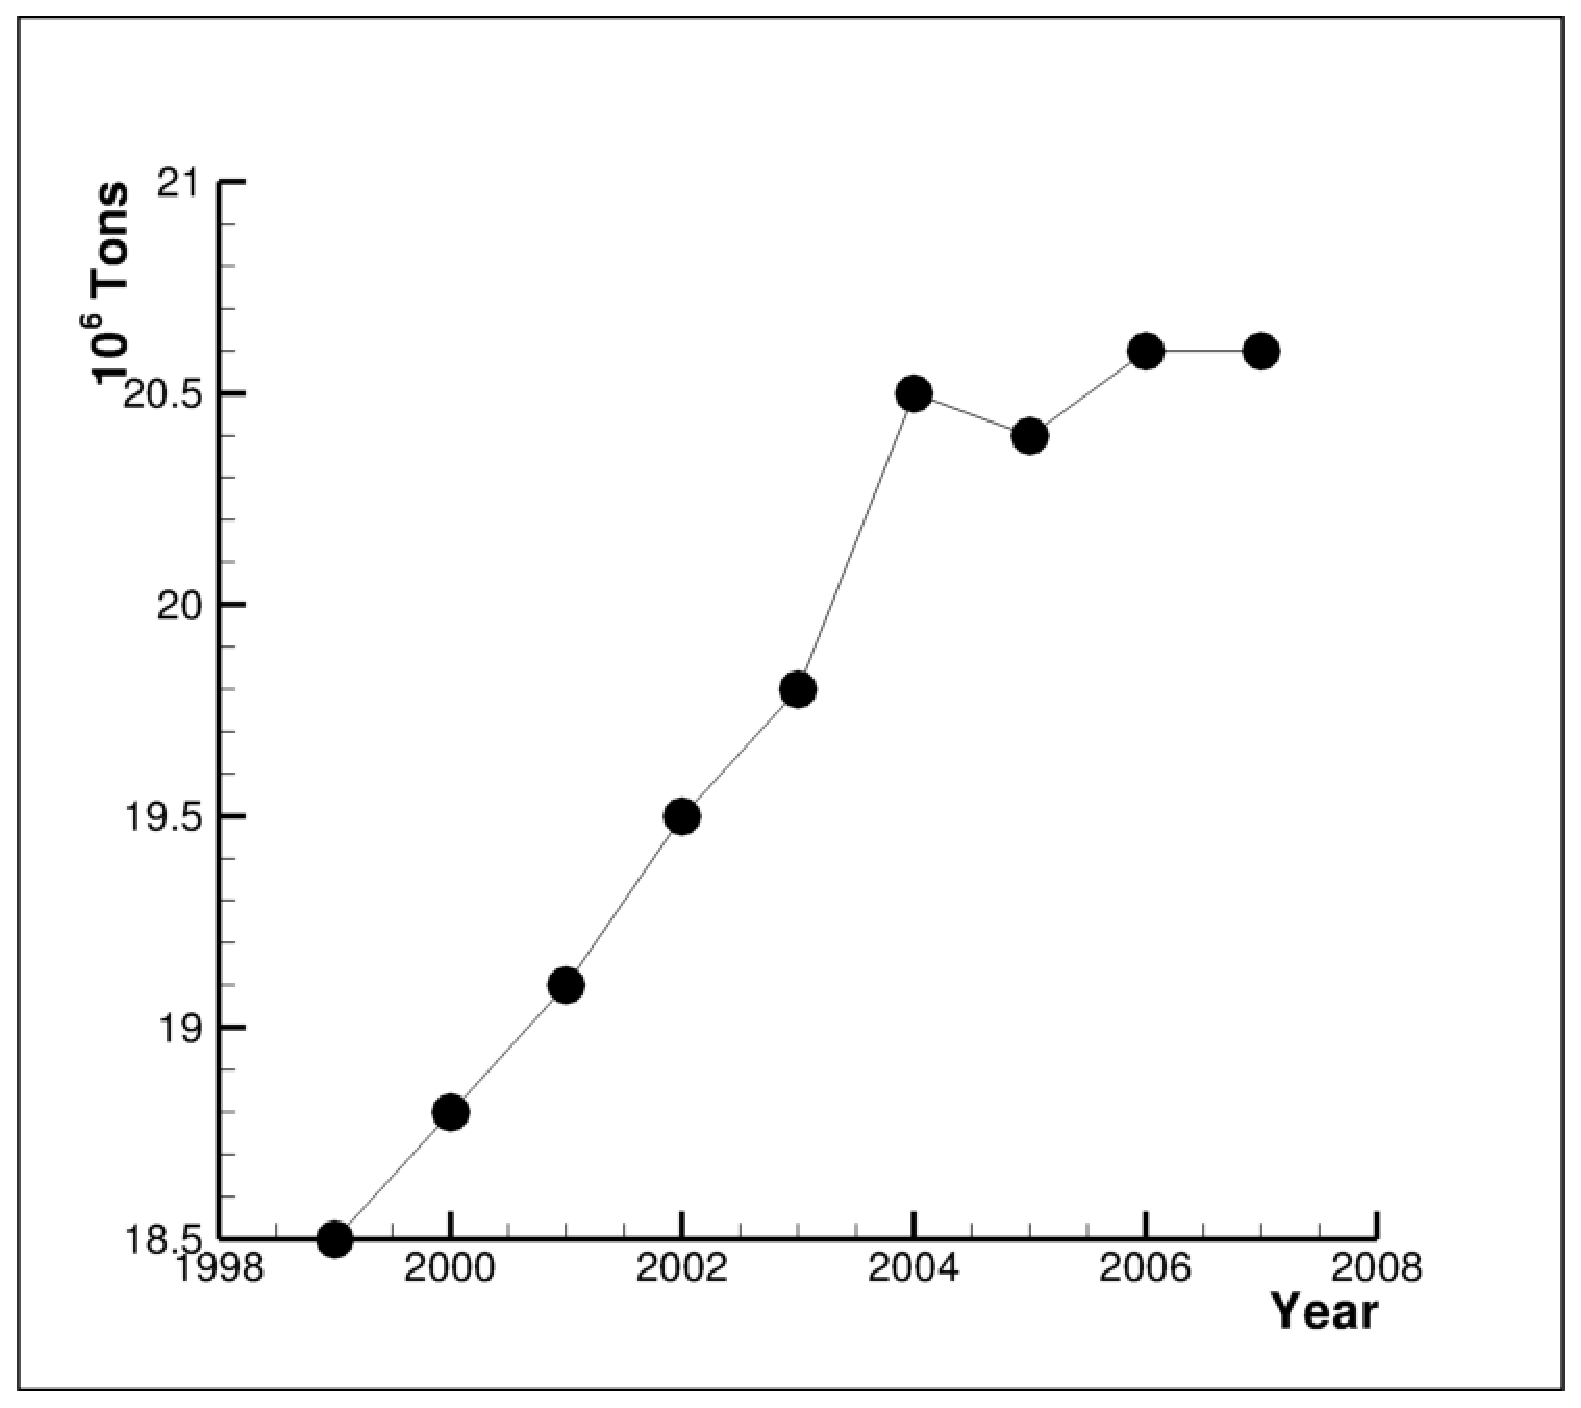
\includegraphics[scale=0.23]{atmosphereDynamic}
				\caption{Динамика выбросов твёрдых веществ в атмосферу \cite{emissionInfoRussian}}
				\label{figure:atmosphereDynamic}
			\end{minipage}
		\end{figure}
		\vspace{-1em}
	
		Для очищения воздуха от твёрдых примесей широкое распространение получили фильтры типа циклон. Циклон представляет собой инерционный пылеуловитель, в котором выделение частиц из воздушной среды происходит, в основном, под действием центробежной силы, возникающей при вращении воздушного потока в корпусе аппарата.
	
		Запылённый воздух входит в циклон через тангенциальный патрубок и, приобретая вращательное движение, опускается винтообразно вниз вдоль внутренних стенок цилиндра и конуса. Небольшая часть этого потока, в котором сконцентрированы пылевые частицы, движется в непосредственной близости от стенок циклона и поступает через пылеотводящее отверстие в пылесборный бункер, где происходит осаждение и накопление пылевых частиц.
	
		В центральной зоне циклона воздушный поток, освобождённый от пыли, поднимается винтообразно вверх и удаляется через выхлопную трубу наружу.
	
		Вследствие вращательного движения воздушного потока в центральной зоне циклона (в конусе, выхлопной трубе и пылесборном бункере) наблюдается пониженное давление.\cite{instructions}
	
		В силу высокой степени закрученности потока, необходимо введение поправок в модели турбулентности для учёта кривизны линий тока. Кроме того, учитывая высокую концентрацию частиц в потоке, в инженерных расчётах необходимо учитывать не только влияние потока на частицы, но также и обратное влияние частиц на поток.
	%Актуальность проблемы
	\subsection*{Цели работы}
		\begin{enumerate}
			\item Реализация $k-\omega-SST$ модели турбулентности с поправкой на кривизну линий тока при помощи открытой интегрируемой платформы для численного моделирования задач механики сплошных сред OpenFOAM.
			\item Реализация с использованием OpenFOAM солвера, имеющего в основе модель идеального газа и учитывающего при этом обратное влияние частиц на поток.
			\item Численное моделирование циклона с учётом обратного влияния частиц на поток и поправки на кривизну линий тока к генерации турбулентности.
		\end{enumerate}
	%Цели работы
%Введение

\newpage
\section{Обзор существующих исследований}
	Циклоны используются для удаления твёрдых частиц из газовых потоков с конца 19 века. Простая конструкция, низкие затраты на производство и обслуживание, а также адаптивность к широкому диапазону рабочих параметров сделали циклоны одними из наиболее часто используемых промышленных фильтров. 
	
		Эффективность циклонов определяется степенью очистки воздуха $\eta$, равной отношению количества частиц данного диаметра, задержанных циклоном к полному числу частиц. В силу того, что принцип работы этих фильтров основан на инерциальных силах, они имеют низкую эффективность для частиц, диаметром менее $5 \mu m$.
	
	Существует огромное количество конфигураций, однако противоточные циклоны с тангенциальным входом \textit{(рисунок \ref{fig:cycloneOverview})} чаще всего используются для очистки воздуха в промышленности. Такая конфигурация описывается девятью безразмерными параметрами \textit{(таблица \ref{tableCyclone})}, отнесёнными к масштабу длины $D$, характеризующему диаметр фильтра \cite{DirgoLeith}.\\
  \begin{minipage}{0.6\textwidth}
    \captionof{table}{Геометрия фильтра}
			\begin{tabular}{l l}
				\hline
				\label{tableCyclone}
				Диаметр цилиндра, & $D$\\
				Диаметр выходной трубы, & $D_e$\\
				Высота входного канала, & $a$\\
				Ширина входного канала, & $b$\\
				Длина выходной трубы, & $h_e$\\
				Полная высота фильтра, & $H$\\
				Высота цилиндра, & $h$\\
				Диаметр нижнего сечения фильтра, & $B$\\
				Высота пылесборника, & $h_d$\\
				Диаметр пылесборника, & $D_d$\\
			\end{tabular}
    \end{minipage}
    \hspace{1em}
  \begin{minipage}{0.35\textwidth}
    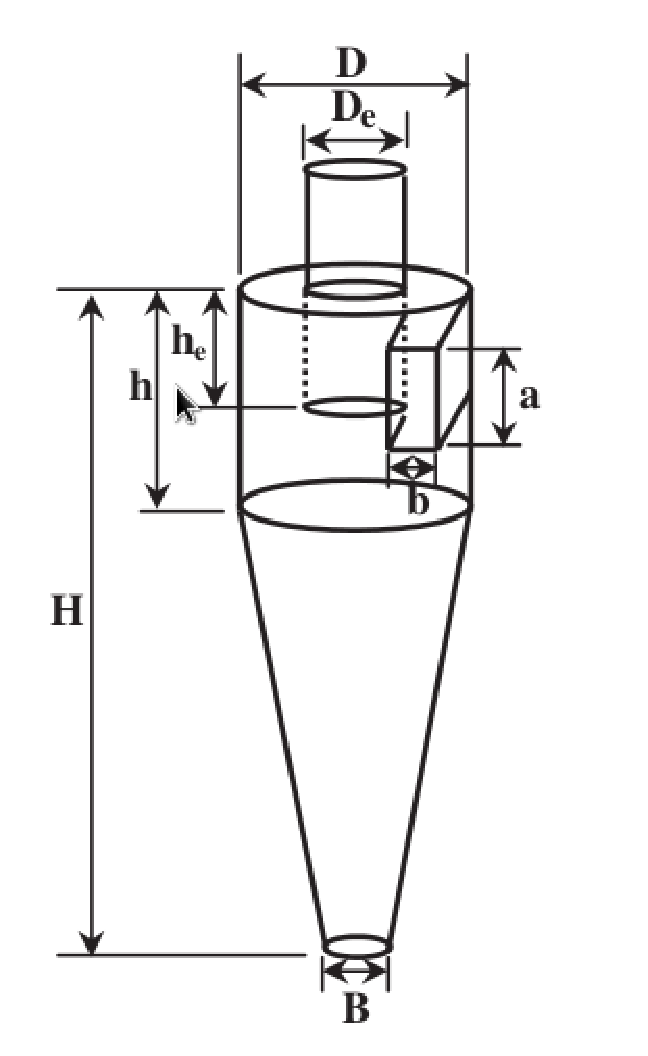
\includegraphics[scale=0.375]{Geometry}
				\captionof{figure}{Схема фильтра}
			    \label{fig:cycloneOverview}
  \end{minipage}
  	\subsection{Теоретические исследования}
	\label{theoreticalOverview}
		\hspace{1em}
		Процесс взаимодействия частиц с несущей фазой очень хорошо описан в книге \cite{Richardson}. Указанная книга предоставляет в явном виде решение большого количества инженерных задач, связанных с течениями дисперсных сред. В конечном виде эти решения являются в большой степени приближёнными, применимы в ограниченном числе случаев и описывают, в основном, общие параметры системы, не давая информации о структуре течения несущей фазы, фокусируясь именно на описании частиц. Тем не менее, теоретические модели, сформулированные в этой книге охватывают широкий диапазон физических процессов, связанных с течениями жидкостей с дисперсными включениями, и могут быть крайне полезны для математического описания таких течений.
		\subsubsection*{Степень очистки}
		\addcontentsline{toc}{subsubsection}{Степень очистки}
		Диргоу и Лейт \cite{DirgoLeith} в своей статье систематизировали теоретические модели, применяемые для расчётов рабочих параметров системы, выделив три основных подхода к описанию циклонов.
			\subparagraph{I. Подход, основанный на времени полёта частиц\\}
			Допустим, частица попадает в циклон на определённом расстоянии от оси фильтра. Частица должна переместиться из этого положения к стенке для того, чтобы быть отфильтрованной. Критический диаметр частицы это такой диаметр, при котором частица перемещается ровно на это расстояние за время пребывания в циклоне. Различные заключения о начальном положении частицы и времени пребывания приводят к различным приближённым решениям. Теория Лэппла \cite{Lapple} является наиболее часто используемым примером такого подхода. Предположим, что пыль, поступающая в циклон, равномерно распределена по всему входному сечению. Лэппл определил критический диаметр частиц для циклонов как диаметр, при котором, частицы, перемещаясь от середины входного сечения до стенки, за время пребывания в циклоне фильтруются с 50\% эффективностью:
			\begin{equation}
				\label{LappleEquation}
				d_{50} = \sqrt{\frac{9\mu b}{2 \pi \rho_p U_i C_d N_t}},
			\end{equation}
			где $\rho_p$ - плотность частиц, $U_i$ - скорость газа на входе в циклон, $\mu$ - динамическая вязкость воздуха, $b$ - ширина входного сечения фильтра, $C_d$ - коэффициент сопротивления.
			
	Число оборотов $N_t$, которые совершает газ внутри фильтра, может быть рассчитано по формуле $N_t = tU_i/\pi D$, а время пребывания $t$ равно отношению объёма циклона к объёмному расходу воздуха $Q$ \cite{Kuo}.
	
	Эффективность для частицы произвольного диаметра $d$ может быть определена из величины отношения этого диаметра к $d_{50}$.
	\begin{figure}[ht]
		\centering
		\includegraphics[scale=0.5]{Lapple}
		\caption{Степень очистки в зависимости от $d/d_{50}$}
		\label{fig:lapple}
	\end{figure}
	На \textit{рисунке \ref{fig:lapple}} показана степень очистки в зависимости от $d/d_{50}$, построенная на основе экспериментов Лэппла. Теодоре и де Паола \cite{Theodore} предлагают для определения степени очистки воздуха использовать следующее соотношение, определённое на основе экспериментов Лэппла:
			\begin{equation}
				\eta = \frac{1}{1 + (d/d_{50})^{-2}}
			\end{equation}
			\subparagraph{II. Подход, основанный на статике частиц\\}
			При таком подходе критический диаметр определяется как диаметр частицы, при котором действующая на частицу центробежная сила полностью компенсируется силой сопротивления. Такие частицы должны бесконечно вращаться вокруг границы ядра фильтра, расположенного под выходным сечением. Сила сопротивления, действующая на более мелкие частицы превышает центробежную силу так, что такие частицы пересекают эту границу и, поднимаясь наверх, вылетают из циклона. Более крупные частицы относятся к стенкам циклона и могут, таким образом, быть отфильтрованы. При таком определении критического диаметра, степень фильтрации растёт от нуля для частиц меньше критического диаметра до единицы для частиц, диаметром больше критического. На практике такое строгое разделение недостижимо из-за флуктуаций скорости, а эффективность для критического диаметра, в среднем, должна быть равной 50\%.
			
			Примером этого подхода может служить теория, предложенная в статье Барта \cite{Barth}. Барт определил границы ядра циклона, как воображаемое продолжение стенок выходной трубы до нижнего сечения фильтра или стенок конуса. При таком определении границы, критическая скорость для осаждения статических частиц выражается формулой
			\begin{equation}
				U^{*}_{ts} = \frac{Qg}{2 \pi h^{*} U^2_t}
			\end{equation}
			Степень очистки для других диаметров частиц определяется через отношение критической скорости произвольных частиц к критической скорости статических частиц
			\begin{equation}
				\frac{U_{ts}}{U^{*}_{ts}} = \frac{\pi h^{*}U^2_t\rho_p d^2}{9 \mu Q},
			\end{equation}
			где $h^{*}$ - высота ядра циклона, которая может быть найдена из геометрических соображений, а $Q$ - расход воздуха через входное сечение фильтра. Тангенциальная скорость газа на границе ядра, определяется, как 
			\begin{equation}
				U_t = U_o\left(\frac{(D_e/2)(D-b)\pi}{2ab\alpha + h^{*}(D-b)\lambda \pi}\right),
			\end{equation}
			где $\lambda = 0.02$ - коэффициент трения, $\alpha = 1-1.2(b/D)$, $U_o$ - скорость газа в выходном сечении, $a$ и $b$ - соответственно, высота и ширина входного сечения \cite{Barth}.
			\begin{figure}[ht]
				\centering
				\includegraphics[scale=0.48]{Barth}
				\caption{Степень очистки в зависимости от $U_{ts}/U^{*}_{ts}$}
				\label{fig:barth}
			\end{figure}
			На \textit{рисунке \ref{fig:barth}} показана зависимость степени очистки от $U_{ts}/U^{*}_{ts}$, построенная Бартом на основе экспериментальных результатов для нескольких конфигураций циклона. Кривая Барта хорошо аппроксимируется выражением
			\begin{equation}
				\eta = \frac{1}{1+ (U_{ts}/U^{*}_{ts})^{-3.2}}
			\end{equation}
	
			\subparagraph{III. Прямой расчёт эффективности очистки\\}

			Последний подход позволяет рассчитать эффективность очистки для любого размера частиц и любой конфигурации циклонов. Кривая степени очистки может быть определена без использования обобщённых кривых, основанных на критическом диаметре. Примерами такого подхода являются теория Лейта-Лихта \cite{LeithLicht} и теория Диетца \cite{Dietz}.
			
			Течение в промышленных циклонах на практике всегда является турбулентным. Модель Лейта-Лихта учитывает влияние турбулентности предполагая, что на любой высоте внутри циклона неосевшая пыль представляет собой равномерную смесь. Среднее время пребывания в циклоне определяется на основе его геометрических размеров и расходе воздуха. Итоговое выражение для степени очистки циклона выглядит следующим образом:
			\begin{equation}
				\eta = 1 - \exp[-2 (C\Psi)^{1/(2n+2)}].
			\end{equation}
			Влияние свойств частиц и газа учитывается в модифицированном инерционном параметре $\Psi$.
			\begin{equation}
				\Psi = \frac{\rho_p d^2 U_i (n+1)}{18 \mu D}.
			\end{equation}
			Здесь $C$ - безразмерный геометрический параметр, который зависит только от конфигурации фильтра:
			\begin{equation}
				\begin{aligned}
					\label{geometricParameterEfficiency}
					&C = \frac{\pi D^2}{ab} \Bigg[ 2 \left\lbrace 1 - \left( \frac{D_e}{D}\right)^2 \right\rbrace\left( \frac{h_e}{D} - \frac{a}{2D} \right) + \\ &+ \frac{1}{3} \left( \frac{h_e + l - h}{D} \right)\left( 1+\frac{d_c}{D} + \frac{d_c^2}{D^2}  \right) + \frac{h}{D} - \left( \frac{D_e}{D} \right)^2\frac{l}{D} - \frac{h_e}{D}\Bigg]			
				\end{aligned}
			\end{equation}
			Истинная длина циклона, $l$ определяется как максимальное расстояние, которое преодолевает вращающийся поток в зоне под выходной трубой. 
			\begin{equation}
				\label{naturalLength}
				l = 2.3D_e\left(\frac{D^2}{ab}\right)^{1/3}.
			\end{equation}
			Диаметр конуса на истинной длине определяется, как
			\begin{equation}
			\label{diameterAtNaturalLength}
				d_c = D - \frac{(D-B)(h_e + l -h)}{H - h}
			\end{equation}
			Если истинная длина превышает $(H-h_e)$, $l$ в уравнениях (\ref{geometricParameterEfficiency}) и (\ref{diameterAtNaturalLength}) заменяется на $(H - h_e)$.
			
			Степень экспоненты, $n = 0.5 \div 0.9$, определяет изменение тангенциальной скорости в радиальном направлении: $U_tr^n = const$. Эмпирическая формула для определения $n$ при произвольном диаметре циклона и заданной температуре газа выглядит следующим образом \cite{Alexander}:
			\begin{equation}
				\label{incrementN}
				n = 1 - \left[ (1-0.67D^{0.14})(T/283)^{0.3} \right]
			\end{equation}
			
			Модель Диетца \cite{Dietz} является модифицированным вариантом модели Лейта-Лихта. Диетц разделяет циклон на три региона -- входной участок, область опускающегося течения и ядро циклона. Предполагается, что под действием турбулентности устанавливается равномерный в радиальном направлении профиль концентрации неотфильтрованных частиц внутри каждого региона. Предполагается также, что происходит обмен частицами между областью опускающегося течения и ядром циклона. Для расчёта эффективности циклона предлагается формула
			\begin{equation}
				\eta = 1 - \left[ K_0 - \sqrt{K_1^2 + K_2^2} \right]\exp{\left[\frac{-\pi (2h_e - a)\rho_p d^2 U_i}{18 \mu ab}\right]},
			\end{equation}
			где 
			\begin{eqnarray}
				K_0 &=& \frac{1}{2}\left[ 1 + \left(\frac{D_e}{D}\right)^{2n}\left(1+\frac{9\mu ab}{ \pi \rho_p l d^2 U_i}\right) \right] \\
				K_1 &=& \frac{1}{2}\left[ 1 - \left(\frac{D_e}{D}\right)^{2n}\left(1+\frac{9\mu ab}{ \pi \rho_p l d^2 U_i}\right) \right] \\
				K_2 &=& \left(\frac{D_e}{D}\right)^{2n}.
			\end{eqnarray}
			Как и в модели Лейта-Лихта, $l$ должна быть заменена на $(H-h_e)$, если $l>(H-h_e)$. Величина $n$ может быть вычислена по формуле (\ref{incrementN}).
	\subsubsection*{Перепад давления}
	\addcontentsline{toc}{subsubsection}{Перепад давления}
		Величина перепада давления, создаваемого циклоном, являясь показателем необратимых потерь энергии, имеет чрезвычайно важное значение, поскольку она непосредственно связана с эксплуатационными расходами. Перепад давления определяется, как разница давлений между входным и выходным сечениями фильтра \cite{Utikar}. Циклоны в этом плане имеют одну важную особенность, которая заключается в наличии радиальной компоненты скорости в выходном сечении фильтра, которая затрудняет определение статического давления в этой области. На практике, разница давлений между входной и выходной границей ниже, чем истинный перепад давления.
		
		Обобщенный вариант формулы для определения давления представляет собой произведение числа Эйлера на скоростной напор:
		\begin{equation}
			\triangle P_{air-only}  = \frac{16ab}{D_e^2} \left( \frac{\rho_g U_i^2}{2} \right).
		\end{equation}
		Для слабо запылённых потоков уравнение записанное с использованием безразмерных геометрических параметров, предложенное Лэпплом является более надёжным:
		\begin{equation}
			\triangle P_{air-only} = \frac{16\left(\frac{a}{D}\right)\left(\frac{b}{D}\right)}{\left(\frac{D_e}{D}\right)^2} \frac{\rho_g U_i^2}{2} = \frac{16\left(\frac{a}{D}\right)\left(\frac{b}{D}\right)}{\left(\frac{D_e}{D}\right)^2}\left(\frac{\rho_g\left(\frac{Q}{ab}\right)^2}{2}\right).
		\end{equation}
		Примечательно, что перепад давления сначала падает с увеличением концентрации дисперсных включений, а потом снова начинает расти, начиная с некоторой, достаточно большой, концентрации примесей \cite{Shrikant}. Для определения перепада давления с учётом концентрации примеси используется уравнение Смольника \cite{Smolik}
		\begin{equation}
			\triangle P_{with-solids} = \triangle P_{air-only} (1-0.02c^{0.6}),
		\end{equation}
		где $c$ - концентрация твёрдых частиц на входе в циклон.
	\subsection{Экспериментальные исследования}
		\hspace{1em}Существует большое количество работ по экспериментальному исследованию течения с искривлёнными линиями тока. Среди них стоит выделить достаточно подробный эксперимент, приведённый в статье Monson et al. \cite{Monson}. Авторы статьи проводят численное и экспериментальное исследование турбулентного течения воздуха в U-образном канале.
		
		Экспериментальному моделированию циклонов также уделено немало внимания. Среди статей, приводящих экспериментальные данные по турбулентному течению в циклонах, можно, опять же, отметить детальное исследование течения в циклоне модели Stairmand, описанное в статье J. Dirgo, D. Leith \cite{DirgoLeith}. В этой статье приведены данные для профилей скорости в нескольких сечениях фильтра для большого диапазона рабочих параметров. К сожалению, авторы используют модифицированную модель фильтра, в которой масштаб $D = 0.375m$ отличается от классического $D = 0.205m$, предложенного в работе Stairmand \cite{Stairmand}, поэтому экспериментальные данные неприменимы к моей работе, в которой рассматривается именно классическая модель фильтра.
	\subsection{Численные исследования}
		\hspace{2em}Численному моделированию течения в циклонах посвящено очень много инженерных исследований.
	%Численные исследования
\newpage
%Обзор существующих моделей

\newpage
\section{Численное моделирование}
	\subsection{Уравнения движения}
		\subparagraph{Уравнение баланса массы\\}
			\begin{equation}
				\frac{\partial \rho}{\partial t} + \frac{\partial}{\partial x_i}(\rho u_i) = 0
			\end{equation}
		\subparagraph{Уравнение баланса импульса\\}
			\begin{equation}
				\frac{\partial \rho u_i}{\partial t} + \frac{\partial}{\partial x_j}(\rho u_iu_j) = - \frac{\partial p}{\partial x_i} + \frac{\partial {\tau_{ij}}_{eff}}{\partial x_j} + {S_u}_i,
				\label{flowEqn}
			\end{equation}
			где ${\tau_{ij}}_{eff}$ - тензор вязких напряжений, выражаемый по формуле
			\begin{equation}
				{\tau_{ij}}_{eff} = \mu_{eff}\left( \frac{\partial u_i}{\partial x_j} + \frac{\partial u_j}{\partial x_i} \right) - \frac{2}{3}\mu_{eff}\frac{\partial u_i}{\partial x_j} \delta_{ij} \quad \mu_{eff} = \mu + \mu_{t}
			\end{equation}
		\subparagraph{Уравнение баланса энтальпии\\}
		\begin{equation}
			\frac{\partial \rho h}{\partial t} + \frac{\partial}{\partial x_j} (\rho u_j h) = \frac{\partial p}{\partial t} + \frac{\partial}{\partial x_j} \left((\alpha + \alpha_t) \frac{\partial h}{\partial x_j}\right) - \frac{\partial}{\partial t}\left(\rho \frac{\vec{V}^2}{2}\right) - \frac{\partial}{\partial x_j}\left(\rho u_j \frac{\vec{V}^2}{2}\right) + S_h,
			\label{thermoEqn}
		\end{equation}
		 где $\alpha$ - коэффициент температуропроводности.
		\subparagraph{Уравнение состояния\\}
			\hspace{2em}При расчётах течений сжимаемой жидкости используется модель идеального газа:
			\begin{equation}
				\frac{p}{\rho} = \frac{R}{M}T, \quad M = 28.966 \frac{g}{mole}
			\end{equation}
		
	\newpage
		\subsection{Модель турбулентности}
		
		Формулировка SST-модели турбулентности, согласно \cite{Menter} (но с учётом поправки на кривизну линий тока), следующая:
		\subparagraph{Уравнение баланса кинетической энергии турбулентности\\}
				\begin{equation}
				\frac{\partial \rho k}{\partial t} + \frac{\partial \rho U_j k}{\partial x_j} = \tilde{P}_k f_{rot} - \beta^* \rho k \omega + \frac{\partial}{\partial x_j}(\Gamma_k \frac{\partial k}{\partial x_j}),
				\end{equation}
				где $f_{rot}$ - поправочный коэффициент Шура-Спалларта к генерации турбулентности, учитывающий криволинейность потока, определяемый в \ref{CC}.
		\subparagraph{Уравнение баланса удельной скорости диссипации\\}
			\begin{equation}
				\frac{\partial \rho \omega}{\partial t} + \frac{\partial U_j \omega}{\partial x_j} = \frac{\gamma}{\nu_t}P_kf_{rot} - \beta\rho\omega^2 + \frac{\partial}{\partial x_j}(\Gamma_{\omega}\frac{\partial \omega}{\partial x_j}) + (1-F_1)2\rho \sigma_{\omega_2}\frac{1}{\omega}\frac{\partial k}{\partial x_j}\frac{\partial \omega}{\partial x_j},
			\end{equation}
			где
			\begin{equation}
				\Gamma_k = \mu + \frac{\mu_t}{\sigma_k}, \quad \Gamma_{\omega} = \mu + \frac{\mu_t}{\sigma_{\omega}}, \quad P_k = \tau_{ij}\frac{\partial U_i}{\partial x_j}
			\end{equation}
			$$
			 \tilde{P}_k = min(P_k, c_1\varepsilon), \quad \mu_t=\rho\frac{a_1 k}{max(a_1\omega, S \cdot F_2)}
			$$
			
			Коэффициент $\phi$ в модели представляет собой функцию от $F_1$: $\phi = F_1\phi_1 + (1-F_1)\phi_2$, где $\phi_1$ и $\phi_2$ соответственно коэффициенты для $k-\omega$ и $k-\varepsilon$ моделей.
			$$
				\sigma_{k1} = 1.176, \quad \sigma_{\omega 1} = 2.0, \quad \gamma_1 = 0.5532 \quad \beta_1=0.075, \quad \beta^*=0.09, \quad c_1 = 10,
			$$
			$$
				\sigma_{k2} = 1.0, \quad \sigma_{\omega 2} = 1.168, \quad \gamma_2 = 0.4403 \quad \beta_2=0.0828, \quad \beta^*=0.09, \quad \kappa = 0.41
			$$
			\begin{eqnarray}
				\nonumber F_1 &=& \tanh{(arg_1^4)}, \quad arg_1 = \min\left[\max\left(\frac{\sqrt{k}}{\beta^*\omega y},\frac{500 \nu}{y^2 \omega} \right), \frac{4\rho\sigma_{\omega 2}k}{CD_{k\omega}y^2}\right] \\ \nonumber CD_{k\omega} &=& \max\left( 2\rho\sigma_{\omega_2}\frac{1}{\omega}\frac{\partial k}{\partial x_j}\frac{\partial \omega}{\partial x_j},10^{-10} \right) \\
				F_2 &=& \tanh{(arg_2^2)}, \quad arg_2 = \max\left(2\frac{\sqrt{k}}{\beta^*\omega y},\frac{500 \nu}{y^2\omega}\right) \\
				\nonumber \tau_{ij} &=& \mu_t\left( \frac{\partial U_i}{\partial x_j} + \frac{\partial U_j}{\partial x_i} - \frac{2}{3}\frac{\partial U_k}{\partial U_k}\right) - \frac{2}{3}\rho k \delta_{ij}
			\end{eqnarray}
	<<<<<<< HEAD
	\subsubsection{Введение поправки на кривизну линий тока}
		\label{CC}
		Наличие членов, явно учитывающих вклад вращения и кривизны линий тока в уравнениях моделей турбулентности цитируется как фундаментальное преимущество моделей Рейнольдсовых напряжений над более простыми моделями турбулентной вязкости \cite{ShurSpallart}. Внесение эффективных изменений в более простые модели может, тем не менее, иметь широкое применение в силу того \cite{CC2}, что для большого класса вычислительных задач модели Рейнольдсовых напряжений пока не доведены до того состояния, в котором они показали бы свою высокую стабильность и точность расчётов \cite{CC3}.
		
		Влияние вращения и кривизны линий тока на турбулентность проявляется наиболее сильно в двух предельных случаях. В тонких сдвиговых течениях с маленькой, по сравнению со скоростью сдвига, скоростью вращения или слабой кривизной линий тока, наблюдается значительное влияние этих эффектов на уровень турбулентных напряжений \cite{Bradshaw}. Другим крайним случаем является однородное сдвиговое течение во вращающейся области, в котором турбулентные пульсации затухают под влиянием сильного вращения \cite{Speziale}. Другой случай сильного вращения это течение в ядре свободного вихря, моделирование которого также даёт плохие результаты при использовании немодифицированных моделей турбулентности \cite{Govindaraju}.
		
		Для учёта влияния кривизны линий тока в моей работе используется поправка на кривизну линий тока, предложенная для модели Spalart-Almaras в \cite{ShurSpallart} и переформулированная применительно к SST модели в \cite{Smirnov}.
		
		В указанной работе рассматривается сдвиговое течение с базовой скоростью, направленной по оси $x$, а все величины меняются, в основном, в направлении $y$. Пусть $U(y)$ - профиль скорости, и пусть $U_y > 0$ так что $\omega_z < 0$. Состредоточимся на проекции тензора Рейнольдсовых напряжений $-\overline{u^{'}v^{'}}$. Вращение с угловой скоростью $\Omega$ вносит вклад $2\Omega(\overline{{u^{'}}^2}-\overline{{v^{'}}^2})$ в эту величину. Если $\overline{{u^{'}}^2} > \overline{{v^{'}}^2}$, величина касательного напряжения возрастает, и наоборот. Таким образом, генерационный член возникает из-за достаточно тонких особенностей тензора Рейнольдсовых напряжений, которые, конечно, не учитываются в моделях турбулентной вязкости.
		
		В случае криволинейности потока, аналогичный член появляется, если уравнения движения записать в криволинейной системе координат, ориентированной по направлению потока, что приводит к появлению ``эффективной скорости вращения'', равной $U/R$, где $R$ - радиус кривизны линий тока ($R$ принимается положительной в случае вогнутых линий тока). $U/R$ может быть записана, как $\frac{\partial v}{\partial x}$, причём $v$ - скорость, направленная перпендикулярно к линиям тока, а $x$ - направление движения. $\frac{\partial v}{\partial x}$ не является Галилеевым инвариантом так как это частная производная по оси, сонаправленной с вектором скорости.
		
		Неравнозначность $\overline{{u^{'}}^2} > \overline{{v^{'}}^2}$ в тонком сдвиговом течении эквивалетна тому, что главные оси тензора Рейнольдсовых напряжений не сонаправлены с главными осями тензора сдвиговых деформаций. Таким образом, при вращении оси тензора напряжений опережают, или отстают от осей тензора скоростей деформации в зависимости от знака $\Omega$. Авторы статьи выдвигают следующую гипотезу: "под влиянием вращения (или кривизны линий тока) турбулентность усиливается, если главные оси тензора Рейнольдсовых напряжений опережают оси тензора скоростей деформации, и наоборот". Эта гипотеза обобщает эффекты вращения и кривизны, давая $\Omega$ и $U/R$ схожие роли.
		
		В слабо закрученном тонком сдвиговом течении направление движения, направление главных осей тензора Рейнольдсовых напряжений и тензора скоростей деформации меняется с одинаковой скоростью, $U/R$. Оси тензора скоростей деформации инвариантны и могут быть использованы в простой модели турбулентности. Это приводит к фундаментальному соотношению, 
		$$
			\frac{D\alpha}{Dt},
		$$
		где $\alpha$ - угол между главными осями тензора скоростей деформации и осями системы координат. Будучи Лагранжевой производной величины, которая определена относительно инерциальной системы координат, $D\alpha/Dt$ является Галилеевым инвариантом. В однородном вращающемся потоке с деформацией, не зависящей от времени, $D\alpha/Dt = \Omega$. В неоднородном потоке выражение гораздо сложнее, и, следуя авторам, для несжимаемого течения
		\begin{equation}
			\frac{D\alpha}{Dt} = \Omega + \frac{1}{2\left( S_{11}^2 + S_{12}^2 \right)} \left[ S_{11} \frac{DS_{12}}{Dt} - S_{12} \frac{DS_{11}}{Dt} \right],
		\end{equation}
		где $S_{ij}$ -- тензор скоростей деформации во вращающейся системе координат. $S_{21}$ и $S_{22}$ не присутствуют в формуле в силу симметричности тензора.
		
		Промежуточные выкладки для трёхмерного случая слишком громоздки, поэтому, приведём только окончательный вариант поправки на кривизну линий тока, предложенный в \cite{Smirnov}, но без учёта вращения.
=======
	\subparagraph{Поправка на кривизну линий тока\\}
		\label{CC}
		Согласно \cite{Smirnov}, формулировка поправочного члена, учитывающего кривизну линий тока, к модели Ментера следующая:\\
>>>>>>> pif/master
		\begin{equation}
				f_{r1}(r^*,\tilde{r}) = 2r^*\left( \frac{1+C_{r1}}{1+ r^*} \right)\left[ 1-C_{r3}\arctan{(C_{r2}\tilde{r})} \right] - C_{r1},
		\end{equation}
		\begin{equation}
				\tilde{r} = 2\Omega_{ik}S_{kj}\frac{DS_{ij}}{Dt}\frac{1}{\Omega D^3}, \quad D^2 = \max(S^2, 0.09 \omega^2),
		\end{equation}
		$$
				S^2 = 2 S_{ij}S_{ij}, \quad \Omega^2 = 2 \Omega_{ij} \Omega_{ij}, \quad r^* = S/\Omega
		$$
		$$
				C_{r1} = 1, \quad C_{r2} = 2, \quad C_{r3} = 1, \quad f_{rot} = \max[\min(f_{r1},1.25),0]
		$$
		%Поправка на кривизну линий тока

	%Модель турбулентности

	\newpage
		\subsection{OpenFOAM}
		\hspace{2em}OpenFOAM — свободно распространяемый инструментарий вычислительной гидродинамики для операций с полями (скалярными, векторными и тензорными). На сегодняшний день является одним из самых известных приложений с открытым кодом, предназначенных для FVM-вычислений.\cite{openfoam}
		Код OpenFOAM, разработан в Великобритании в компании \textit{OpenCFD, Limited}, и используется многими промышленными предприятиями более 12 лет. Свое название и идеологию построения код берет от предшественника FOAM (Field Operation And Manipulation), который является закрытым и продолжает развиваться параллельно с OpenFOAM. Первоначально, программа предназначалась для прочностных расчетов и в результате многолетнего академического и промышленного развития на сегодняшний момент позволяет решать следующие задачи:
	\begin{itemize}
		\item Прочностные расчеты;
		\item Гидродинамика сжимаемых и несжимаемых сред. Для моделирования турбулентных течений возможно использование RANS и LES - методов. Возможно решение дозвуковых, околозвуковых и сверхзвуковых задач;
		\item Задачи теплопроводности в твёрдом теле;
		\item Течения многофазных сред;
		\item Течения химически реагирующих смесей;
		\item Задачи, связанные с деформацией расчётной сетки;
		\item Распараллеливание расчёта как в кластерных, так и многопроцессорных системах.
	\end{itemize}

	В основе кода лежит набор библиотек, предоставляющих инструменты для решения систем дифференциальных уравнений в частных производных. Рабочим языком кода является C++. В терминах данного языка большинство математических операторов в программном коде уравнений может быть представлено в удобочитаемой форме, а метод дискретизации и решения для каждого оператора может быть выбран уже пользователем в процессе расчёта. Таким образом, в коде полностью инкапсулируются и разделяются понятия расчетной сетки, дискретизации основных уравнений и методов решения алгебраических уравнений.
	%OpenFOAM

	\newpage
		\newpage
	\subsection{Метод конечных объёмов}
		Суть метода заключается в разбиении расчётной области на множество непересекающихся конечных объёмов (ячеек), для каждого из которых записывается интегральная формулировка законов сохранения.
		\begin{figure}
			\centering
			\includegraphics[scale=0.5]{twoCells}
			\caption{Схематическое изображение двух соседних ячеек}
			\label{fig:twoCells}
		\end{figure}
		\subsubsection*{Дискретизация уравнений}
		\addcontentsline{toc}{subsubsection}{Дискретизация уравнений}
		\begin{figure}[ht]
			\begin{minipage}{0.43\linewidth}
				\includegraphics[scale=0.5]{controlVolume}
				\vspace{-2em}
				\caption{Контрольный объём}
				\label{fig:volume}
			\end{minipage}
			\hspace{-1em}
			\begin{minipage}{0.6\linewidth}
				\vspace{-2em}
				Пусть через контрольный объём $V$ \textit{(рисунок \ref{fig:volume})}, ограниченный контрольной поверхностью $S$, $\vec{\delta S} = \vec{n} \delta S$, проходит жидкость со скоростью $\vec{U}$. Выделим бесконечно малый объём $\delta V$. 
			\end{minipage}
		\end{figure}
		Рассмотрим скалярную величину $\Phi$ - плотность распределения некоторой физической величины на единицу массы. Тогда, с учётом того, что $\rho \delta V = \delta m$, в объёме $\delta V$ содержится $\rho \delta V \Phi$ этой физической величины. Уравнение сохранения для этой величины запишется, как
		\begin{equation}
			\frac{\partial}{\partial t} \int_V \rho \Phi \delta V + \oint_S \left( \rho \vec{U} \Phi + \vec{q}_{\Phi}  \right)\cdot \vec{\delta S} = \int_V \rho S_{\phi} \delta V,
			\label{transportEquation}
		\end{equation}
		где $S_{\Phi}$ - суммарная плотность источников, а $\vec{q}_{\Phi}$ -- дифузионный поток. Это уравнение применяется к каждому контрольному объёму. Задача заключается в сведении уравнения (\ref{transportEquation}) к процедуре алгебраического характера.
		
		Введём точку $C$ -- центр ячейки \textit(рисунок \ref{fig:twoCells}) и применим теорему о среднем к объёмному интегралу:
		\begin{figure}[h]
			\begin{minipage}{0.43\linewidth}
				\includegraphics[scale=0.5]{meanValueTheorem}
				\label{fig:meanValueTheorem}
			\end{minipage}
			\hspace{-1em}
			\begin{minipage}{0.6\linewidth}
				\begin{equation}
					\int_a^b fdx \approx f(x_c) \cdot (b-a)
				\end{equation}
				\begin{equation}
					V \frac{\partial \left(\rho \Phi\right)_c}{\partial t} + \oint_S \left( \rho \vec{U} \Phi + \vec{q}_{\Phi}  \right)\cdot \vec{\delta S} = V \left( \rho S_{\Phi} \right)_c
				\end{equation}
				\vspace{2em}
			\end{minipage}
		\end{figure}
			\vspace{-1em}
					
			Пусть контрольная поверхность состоит из граней, то есть имеется огранённый объект. Тогда
			\begin{equation}
				\oint\left(\rho \vec{U} \Phi + \vec{q}_{\Phi} \right) \cdot \vec{\delta S} = \sum_f \int_{S_f} \left(\rho \vec{U} \Phi + \vec{q}_{\Phi} \right) \cdot \vec{\delta S},
			\end{equation}
			где $f$ -- номер грани.
			\begin{equation}
				\int_{S_f} \left(\rho \vec{U} \Phi + \vec{q}_{\Phi} \right) \cdot \vec{\delta S} \approx \left(\rho \vec{U} \Phi + \vec{q}_{\Phi} \right)_f \cdot \vec{S}_f,
			\end{equation}
			где индекс $f$ в выражении $\left(\rho \vec{U} \Phi  + \vec{q}_{\Phi}\right)_f$ означает, что это значение вычисляется в центре грани, а $\vec{S}_f = \vec{n} S_f$. В итоге мы получаем алгебраическое выражение
			\begin{equation}
				V\frac{\partial \left( \rho \Phi \right)_c}{\partial t} + \sum_f \left( \rho \vec{U} \Phi + \vec{q}_{\Phi} \right)_f \cdot \vec{S}_f = V \left( \rho S_{\Phi} \right)_c
			\end{equation}
		\subparagraph{Расчёт диффузионных потоков}
		\begin{equation}
			\int_V \nabla \cdot \left( \Gamma \nabla \Phi \right) \delta V = \int_S \vec{\delta S} \cdot (\Gamma \nabla \Phi) = \sum_f \Gamma_f \vec{S}_f \cdot (\nabla \Phi)_f
		\end{equation}
		\subparagraph{Расчёт ковективных потоков}
		\begin{equation}
			\int_V \nabla \cdot (\rho \vec{U} \Phi) \delta V = \int_S \vec{\delta S} \cdot (\rho \vec{U} \Phi) = \sum_f \vec{S}_f \cdot (\rho \vec{U})_f \Phi_f = \sum_f F \Phi_f
		\end{equation}
		Значение $\Phi_f$ на грани ячейки может быть определено с использованием различных схем:
		
		\textit{Центральная схема (CD)}
		\begin{equation}
		\Phi_f = \beta \Phi_N + (1-\beta)\Phi_C,
		\end{equation}
		где $\beta=\frac{\vec{|CM|}}{\vec{|CM|} + \vec{|NM|}}$ - коэффициент интерполяции, а точка $M$ -- центр грани $f$.
		
		Для коррекции на скошенность ячеек, когда центр грани $f$ не совпадает с пересечением грани $f$ и вектора $\vec{|CP|}$ (точка $M^{'}$), разложим $\Phi_f$ в ряд Тейлора в окрестности точки $M$ и удержим только первые два слагаемых:
		\begin{equation}
			\Phi_M = \Phi_{M^{'}} + \nabla \Phi_{M^{'}} \cdot \vec{M^{'}M} + O\left(\left(M-M^{'}\right)^2\right)
		\end{equation}
		
		\textit{Противопоточная схема (UD)}
		\begin{equation}
			\begin{aligned}
				\Phi_f = \Bigg\{	\begin{array}{l}
					\Phi_P, \quad \text{если } F \geq 0 \\
					\Phi_N, \quad \text{если } F < 0
				\end{array}
			\end{aligned}
		\end{equation}
		
		\textit{Смешанные схемы}
		\begin{equation}
			\Phi_f = \left(1-\gamma\right)(\Phi_f)_{UD} + \gamma (\Phi_f)_{CD},
		\end{equation}
		где коэффициент $\gamma$ меняется в зависимости от конкретной схемы.
		
		\subparagraph{Расчёт градиентов\\}
		
		    Значение градиента может быть вычислено двумя различными способами.
			
			\textit{Метод Гаусса}
			\begin{equation}
				\int_V \nabla \Phi \delta V = \int_S \vec{\delta S} \Phi = \sum_f \vec{S}_f \Phi_f
			\end{equation}
			
			\textit{Метод наименьших квадратов}
			
			Значение $\Phi$ в точке $C$ может быть экстраполировано в соседнюю ячейку с центром в точке $N$ с использованием градиента в точке $C$. Экстраполированное значение в точке $N$ сравнивается с актуальным значением в этой точке и рассчитывается ошибка в определении $\Phi$. Если мы теперь минимизируем сумму квадратов взвешенных ошибок во всех соседних ячейках по отношению к градиенту, значение градиента будет аппроксимировано достаточно точно. Таким образом, вычислив сначала значение тензора
			\begin{equation}
				\mathbf{G} = \sum_N \omega_N^2 (\vec{CN}\vec{CN}),
			\end{equation}
			где весовая функция $\omega = 1/\vec{|CN|}$, а индекс $N$ означает суммирование по всем соседним граням, мы сможем вычислить значение градиента в точке $C$:
			\begin{equation}
				(\nabla \Phi)_C = \sum_N \omega_N^2 \mathbf{G}^{-1} \cdot  (\Phi_N - \Phi_C).
			\end{equation}
	%Метод конечных объёмов

%Численное моделирование

\newpage
\section{Результаты}
\subsection{Валидация модели турбулентности с поправкой на кривизну линий тока}
\label{UDUCTComparison}

Эффективность поправки на кривизну линий тока к модели Ментера можно проверить, если сравнить результаты расчётов плоского течения в U-образном канале, выполненных при помощи модифицированной модели турбулентности, с экспериментальными данными Монсона и др., приведёнными в статье Монсона \cite{Monson}.

В \textit{таблице \ref{tableUDuct}} представлены геометрические параметры канала и граничные условия. Стенки полагаются адиабатическими, а на выходной границе задаётся постоянное статическое давление $P_{out} = 1.15 atm$. На входной границе задаётся неоднородный профиль скорости и турбулентных характеристик, полученный из решения задачи о развитом турбулентном течении в плоском канале. При таких параметрах число Рейнольдса $Re = 10^5$.

\begin{figure}[h]
	\begin{minipage}{0.5\linewidth}
		\captionof{table}{Геометрия канала}
			\begin{tabular}{r l}
				\hline
				\label{tableUDuct}
				Высота & $H=3.81cm$ \\
				Длина канала & $L = 10H$ \\
				Внутренний радиус & $R_i = 1.91cm$ \\
				Внешний радиус & $R_o = 5.72cm$ \\
				Ср. скорость на входе & $U_{in} = 30.1 m/s$ \\
				Температура на входе & $T_{in} = 264 K$ \\
			\end{tabular}
	\end{minipage}
	\hspace{2em}
	\begin{minipage}{0.4\linewidth}
		\begin{flushright}
		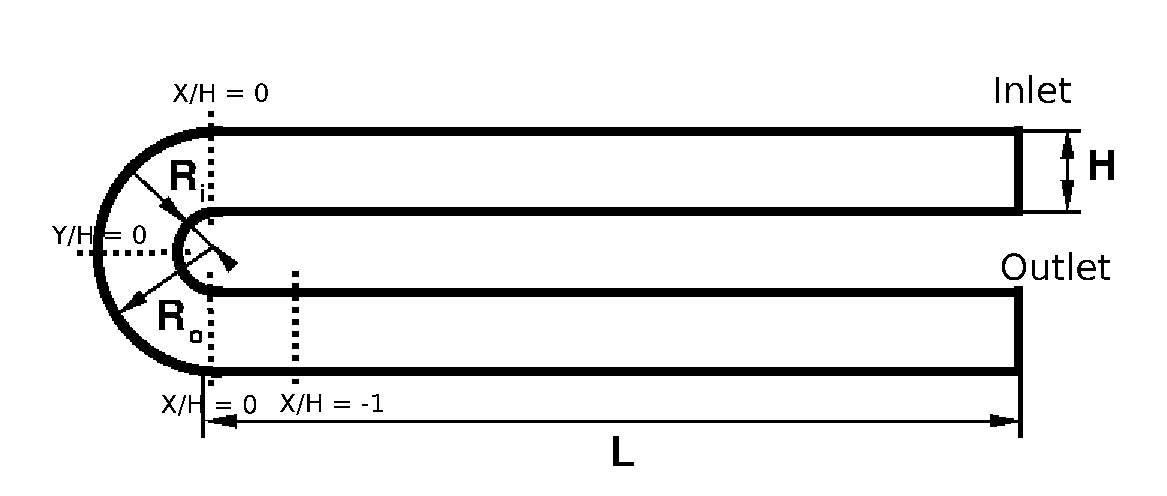
\includegraphics[scale=0.4]{UDuct}
		\caption{Геометрия канала}
		\end{flushright}
	\end{minipage}
\end{figure}
\newpage
\begin{figure}[h]
	\centering
	\includegraphics[scale=0.4]{uDuctyplus}
	\caption{Величина $y^{+}$ первой пристенной ячейки на внешней и внутренней стенках}
	\label{fig:uDuctyplus}
\end{figure}
\clearpage

Величина $y^{+}$ \textit{(рис. \ref{fig:uDuctyplus})} для первой пристенной ячейки лежит в пределах $10 \div 80$, что вполне приемлемо для расчётов с использованием автоматических пристеночных функций.

Перейдём теперь непосредственно к сравнению результатов расчёта с экспериментами Монсона и решением в Fluent с использованием встроенной в него поправки к модели Ментера для учёта кривизны линий тока. Для сравнения выбрано 5 поперечных сечений канала - $x/H=-1$, $x/H = 1$, $x/H = 0$ (верхний канал), $x/H = 0$ (нижний канал) и $y/H=0$.
\begin{figure}[h]
	\centering
	\includegraphics[scale=0.55]{yh0}
	\caption{Профиль поперечной скорости в сечении $y/H=0$}
	\label{fig:y0}
\end{figure}
\begin{figure}[ht]
	\begin{minipage}{0.475\linewidth}
		\includegraphics[scale=0.33]{xh0up}
		\caption{Профиль продольной скорости в сечении $x/H=0$ (верхний канал)}
		\label{fig:x0up}
	\end{minipage}
	\hspace{0.5em}
	\begin{minipage}{0.475\linewidth}
		\includegraphics[scale=0.33]{xh0down}
		\caption{Профиль продольной скорости в сечении $x/H=0$ (нижний канал)}
		\label{fig:x0down}
	\end{minipage}
\end{figure}
\begin{figure}[ht]
	\vspace{-1em}
	\begin{minipage}{0.475\linewidth}
		\includegraphics[scale=0.33]{xh1up}
		\caption{Профиль продольной скорости в сечении $x/H=-1$}
		\label{fig:x1up}
	\end{minipage}
	\hspace{0.5em}
	\begin{minipage}{0.475\linewidth}
		\includegraphics[scale=0.33]{xh1down}
		\caption{Профиль продольной скорости в сечении $x/H=1$}
		\label{fig:x1down}
	\end{minipage}
\end{figure}
\clearpage

Для начала, стоит сказать, что профили продольной скорости на участке перед поворотом \textit{(рисунки \ref{fig:x0up} и \ref{fig:x1up})}, полученные в Fluent и OpenFOAM совпадают с точностью до толщины линии и очень хорошо соответствуют экспериментальному течению. Это говорит о том, что базовая модель Ментера, выбранная для введения поправки, правильно предсказывает течение на прямолинейном участке канала.

Из \textit{рисунков \ref{fig:y0}, \ref{fig:x0down} и \ref{fig:x1down}} видно, что профили скорости, полученные с использованием модифицированной модели Ментера гораздо ближе к экспериментальным данным в пристеночной области криволинейной части канала, чем решение, полученное с использованием стандартной модели. Поправка, при этом, как и следовало ожидать, не влияет на прямолинейное течение в зоне перед поворотом \textit{(рисунки \ref{fig:x0up}, \ref{fig:x1up})}.

Влияние поправки сильнее всего заметно на выпуклой внутренней стенке, генерация турбулентности на которой в немодифицированной модели Ментера занижена. Надо заметить, что результаты, полученные с использованием OpenFOAM при этом лучше согласуются с экспериментами Монсона, чем результаты расчётов в Fluent. Это, однако же, несправедливо для вогнутой внешней стенки. Здесь результаты расчётов в Fluent, наоборот, ближе к экспериментальному профилю. Видно также, что на вогнутой стенке ни в Fluent, ни в OpenFOAM поправка практически не влияет на течение.

В целом, очевидно достаточно сильное положительное влияние введённой поправки, учитывающей кривизну линий тока, на результаты расчётов.
\newpage
\subsection{Расчёт циклона}
\paragraph{Постановка задачи\\}
\addcontentsline{toc}{paragraph}{Постановка задачи}
В задаче рассматривается турбулентное течение вязкого газа с дисперсными включениями в циклоне модели Stairmand c учётом влияния дисперсной фазы на исходное течение. Геометрические параметры циклона представлены в \textit{таблице \ref{cycloneGeomPar}}.

  \begin{minipage}{0.6\textwidth}
    \captionof{table}{Геометрия фильтра}
    \label{cycloneGeomPar}
			\begin{tabular}{l l}
				\hline
				\label{geometrytable}
				Диаметр цилиндра, $D$ & $0.205m$ \\
				Диаметр выходной трубы, $D_e$ & $0.5D$ \\
				Высота входного канала, $a$ & $0.5D$ \\
				Ширина входного канала, $b$ & $0.2D$ \\
				Длина выходной трубы, $h_e$ & $0.75D$ \\
				Полная высота фильтра, $H$ & $4.0D$ \\
				Высота цилиндра, $h$ & $1.5D$ \\
				Диаметр нижнего сечения, $B$ & $0.36D$ \\
				Высота пылесборника, $h_d$ & $0.25D$ \\
				Диаметр пылесборника, $D_d$ & $0.75D$ \\
			\end{tabular}
    \end{minipage}
    \hspace{1em}
  \begin{minipage}{0.35\textwidth}
    \includegraphics[scale=0.45]{cycloneGeometryTeta}
	\captionof{figure}{Схема фильтра}
	\label{fig:cycloneGeometryScheme}
  \end{minipage}
  \vspace{1em}
	
	Течение исследуется для 4 различных скоростей на входе, а также для трёх диаметров частиц. Граничные условия для задачи описаны в \textit{таблице \ref{cycloneBC}}, а на \textit{рисунке \ref{fig:cycloneMesh}} показана сетка расчётной области.
	
\begin{minipage}{0.6\textwidth}
    \captionof{table}{Граничные условия}
    \label{cycloneBC}
	\begin{tabular}{c}
		\hline
		\label{geometrytable}
		Скорость на входе, $U_{in}=$  $5, 10, 15, 20 m/s$ \\
		Температура на входе, $T_{in}=$  $300 K$ \\
		Температура частиц, ${T_p}_{in}=$  $300 K$ \\
		Скорость частиц на входе, ${U_p}_{in} = U_{in}$ \\
		Давление на выходе, $P_{out}=$  $1atm$ \\
		Тепловой поток на стенках, $q_w=$  $0$ \\
		Диаметр частиц, $d_p=$ $10^{-5}m, 10^{-6}m, 10^{-7}	m$\\
	\end{tabular}
\end{minipage}
\hspace{1em}
\begin{minipage}{0.35\textwidth}
    \includegraphics[scale=0.45]{meshCyclone}
	\captionof{figure}{Сетка расчётной области}
	\label{fig:cycloneMesh}
\end{minipage}
\vspace{1em}  
  \paragraph{Методические исследования\\}
  \addcontentsline{toc}{paragraph}{Методические исследования}

  Для исследования сеточной сходимости решения, расчёты задачи с  $U_{in} = 20m/s$ проводились на сетках 29380 ячеек, 96256 ячеек и 179552 ячейки. Сравнение профилей скорости вдоль двух отрезков, $1:$ $\left\{\left(0, 0, -0.3\right),\left(0.09, 0, -0,3\right)\right\}$ и $2:$ $\left\{\left(0, 0, -0.3\right),\left(0, 0.09, -0,3\right)\right\}$, представлены на \textit{рисунках \ref{fig:cycloneMeshIndependence1} -  \ref{fig:cycloneMeshIndependence4}}.
 \begin{figure}[h]
	\vspace{-1em}
	\begin{minipage}{0.475\linewidth}
		\includegraphics[scale=0.33]{cycloneMeshIndependence1}
		\caption{Профили $V_y$ вдоль прямой $1$}
		\label{fig:cycloneMeshIndependence1}
	\end{minipage}
	\hspace{0.5em}
	\begin{minipage}{0.475\linewidth}
		\includegraphics[scale=0.33]{cycloneMeshIndependence2}
		\caption{Профили $V_z$ вдоль прямой $1$}
		\label{fig:cycloneMeshIndependence2}
	\end{minipage}
\end{figure}

 \begin{figure}[h]
	\vspace{-1em}
	\begin{minipage}{0.475\linewidth}
		\includegraphics[scale=0.33]{cycloneMeshIndependence3}
		\caption{Профили $V_x$ вдоль прямой $2$}
		\label{fig:cycloneMeshIndependence3}
	\end{minipage}
	\hspace{0.5em}
	\begin{minipage}{0.475\linewidth}
		\includegraphics[scale=0.33]{cycloneMeshIndependence4}
		\caption{Профили $V_z$ вдоль прямой $2$}
		\label{fig:cycloneMeshIndependence4}
	\end{minipage}
\end{figure}
\clearpage
Видно, что решение на самой грубой сетке (29380 ячеек) сильно отличается от решения на более подробных сетках. В то же время, решение на сетках 96256 ячеек и 179552 ячейки отличаются менее, чем на 5\%, так что, сетки в 96256 ячеек вполне достаточно для получения сеточно-независимого решения. Кроме того, решения в Fluent и OpenFOAM прекрасно соответствуют друг другу -- профили скорости на \textit{рисунках \ref{fig:cycloneMeshIndependence1} -  \ref{fig:cycloneMeshIndependence4}} для Fluent и OpenFOAM практически неотличимы для подробных сеток.

\begin{figure}[h]
	\centering
	\includegraphics[scale=0.4]{yplusCyclone}
	\caption{Величина $y^{+}$ первой пристенной ячейки на внешней и внутренней стенках циклона}
	\label{fig:cycloneyPlus}
\end{figure}

На \textit{рисунке \ref{fig:cycloneyPlus}}, проиллюстрировано распределение величины $y^{+}$ первой пристенной ячейки, построенное вдоль образующих внешних и внутренных стенок, для углов $\theta=0^o$ и $\theta=180^o$ (отмечены на \textit{рисунке \ref{fig:cycloneGeometryScheme}} пунктирными линиями). Из графиков видно, что в большей части области величина $y^{+}$ лежит в пределах $10 \div 90$, что вполне адекватно для использования модели Ментера с автоматическими пристеночными функциями.


\newpage
<<<<<<< HEAD
\section*{Заключение}
\addcontentsline{toc}{section}{Заключение}

В ходе исследования была рассмотрена задача о турбулентном течении газа с дисперсными включениями в фильтре-циклоне при разных значениях скорости потока и различных диаметрах частиц.

Для проведения расчётов в OpenFOAM был имплементирован поправочный коэффициент Шура-Спалларта для учёта влияния кривизны линий тока на турбулентные характерестики. Верификация модели производилась на задаче о турбулентном течении воздуха в U-образном канале и показала явный положительный эффект на результаты расчётов по сравнению с немодифицированной SST-моделью. Результаты расчётов хорошо согласуются с экспериментальными данными Монсона.

Расчёт циклона также показал положительное влияние введённой поправки на профили скорости. 

Сравнение результатов расчётов, выполненных при помощи введённого в OpenFOAM солвера и Fluent показало отличное соответствие решений друг другу. Анализ влияния дисперсных включений на основной поток позволил заключить, что этим влиянием в исследуемой задаче, по большому счёту, можно пренебречь.

Проведено сравнение результатов расчётов с экспериментальными данными Диргоу и Лейта для степени очистки, которое показало хорошее согласие как с экспериментами, так и с теорией, которую эти эксперименты подтверждают. Показана эффективность циклонов для очищения газа от твёрдых частиц диаметром $\sim 10^{-6}m$. Выявлено, что при уменьшении скорости течения, эффективность рассматриваемой конфигурации циклона заметно понижается. Такая же закономерность имеет место и при уменьшении диаметра частиц. Выяснено, что для фильтрации частиц, диаметром меньше $\approx 10^{-7}m$, циклон непригоден так как степень очистки при этом становится меньше 30\%.
=======
%!TEX root = Dissertation.tex
>>>>>>> pif/master

\newpage
\thispagestyle{plain}
\bibliographystyle{plain}
\bibliography{dimbib}
\end{document}
